% !TEX root =../main.tex

\chapter{Implementierung (Minimaler Prototyp) (5 Seiten)}

In dieser Kapitel kann wir ein „ Instanz“ machen. Angenommen, der Nutzer A will ein Computer bei online Shops kaufen, er besitzt nicht Die Erkenntnisse von Hardware und Software, die Parameter von Konfiguration ist ihm Schwer , Er braucht die Hilfe von anderer Leute.

\begin{description}
\item[Schritt 1:] Nutzer A loggt unser Webshop ein, sucht nach „ Computer“.

\item[Schritt 2:] Viele unterschiedliche Computer erscheinen auf den Bildschirm, durch Vergleich von Aussehen hat Nutzer A 3 Marke davon ausgewählt. Er will mit den 3 Verkäufer von den Marke Kontakt machen und nachfragen, wer kann das niedrigste Rabatt anbieten.
\end{description}

Jetzt erzielen die Kommunikation mittels PHP.

In Listing \vref{lst:hello-world} ist dargestellt, wie ein Online-Chat in PHP implementiert werden kann.

% TODO: Quellcode einfügen.

\begin{lstlisting}[language=PHP, caption={Online-Chat in PHP}, label=lst:php-chat]
// socket-resource und die Info vom Nutzer speichern

$connected sockets = array();
// ...
\end{lstlisting}

Seine Nachfrage nehmt in 2 Sekunden bei REAL-Time API die Antwort, zwei Verkäufer aus Dell und Acer versprechen, sie können ein attraktives Rabatt anbieten.

\begin{description}
\item[Schritt 3:] Nutzer A entscheiden, ein Computer von DELL und Acer wird ausgewählt. Er will die Hardware und Komponenten vergleichen. Die Tochter ‘ s Ex Ehemann B von seinem Onkel‘s Cousin ist ein Hardwaretechniker. Nutzer A will die Hilfe von B bekommen.

\item[Schritt 3.1:] Die Kontakt List öffnet, neue Kontaktperson hinzufügen. Der Telefonnummer von B eingeben.

\item[Schritt 3.2:] \glqq{}Commit\grqq{} zu B senden, A ist glücklich wegen guter Freundschaft bestätigt B durch sein Handy SMS.
\end{description}

Die Verbindung zwischen Network und Mobile Smartphone:

Netzwerkstruktur

Im Gegensatz zu herkömmlichen Telekommunikationsdienstnetzwerken müssen wir nicht nur Server, sondern auch zentralisierte Server registrieren und Benutzerknoten in normale Knoten und Superknoten unterteilen. Registrierungsserver Systemverbindungsstruktur wie gezeigt Schematisch

\begin{figure}[htbp]
	\centering
	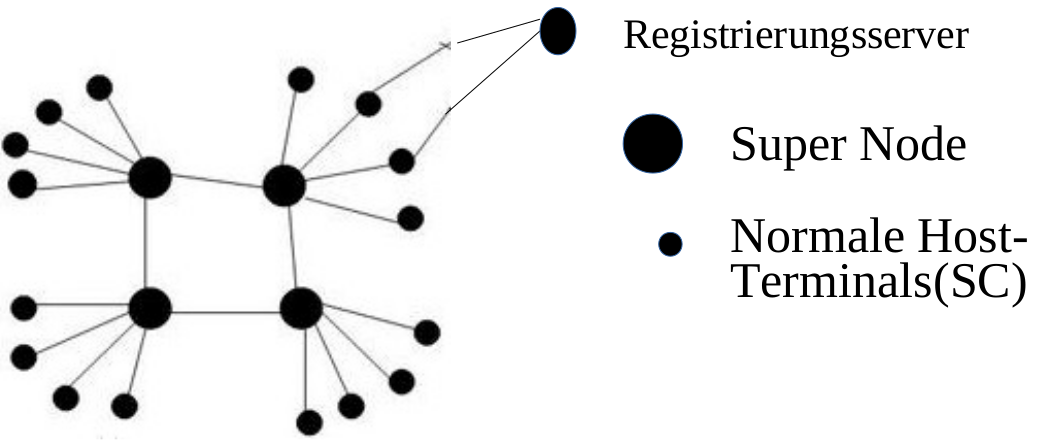
\includegraphics[width=0.4\textwidth]{bilder/telekommunikation-schema.png}
	\caption{Telekommunikation Schematisch}
	\label{fig:telekommunikation}
\end{figure}

Der Registrierungsserver ist ein Gerät, das gewartet werden muss.Es ist verantwortlich für das Registrieren des Clients, das Speichern und Verwaltenvon Benutzernamen und Kennwortinformationen.Wenn sich der Benutzer beim System anmeldet, wird der Benutzer authentifiziert. Der Registrierungsserver muss außerdem die globale Eindeutigkeit des Benutzernamens prüfen und garantieren.

Normale Knoten, dh normale Host-Terminals, müssen Online-Store-Anwendungen herunterladen, um Sprachanrufe und Textnachrichten bereitstellen zu können.

Der Supernode ist tatsächlich ein gewöhnlicher Knoten, der bestimmte Anforderungen erfüllt: Diese Anforderungen umfassen eine öffentliche Netzwerkadresse, eine ausreichende CPU, ausreichend Speicherplatz und eine ausreichende Netzwerkbandbreite. Mit anderen Worten, jedes geeignete Host-Terminal kann ein Super-Knoten werden, vorausgesetzt, die Anwendung wird geladen.


\section{Prozessmodell zur Beschreibung des Ablauf von Kaufen}

\begin{figure}[htbp]
	\centering
	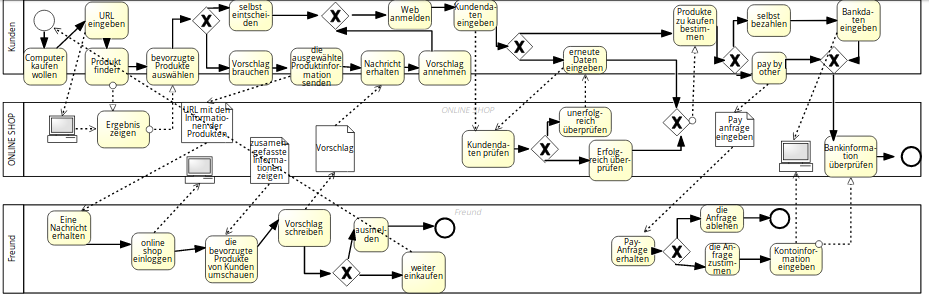
\includegraphics[width=1\textwidth]{bilder/bpmn-ablauf-kaufen.png}
	\caption{Ablauf des Kaufprozess}
	\label{fig:bpmn-ablauf-kaufen}
\end{figure}


\section{Freunde einladen}

\begin{figure}[htbp]
	\centering
	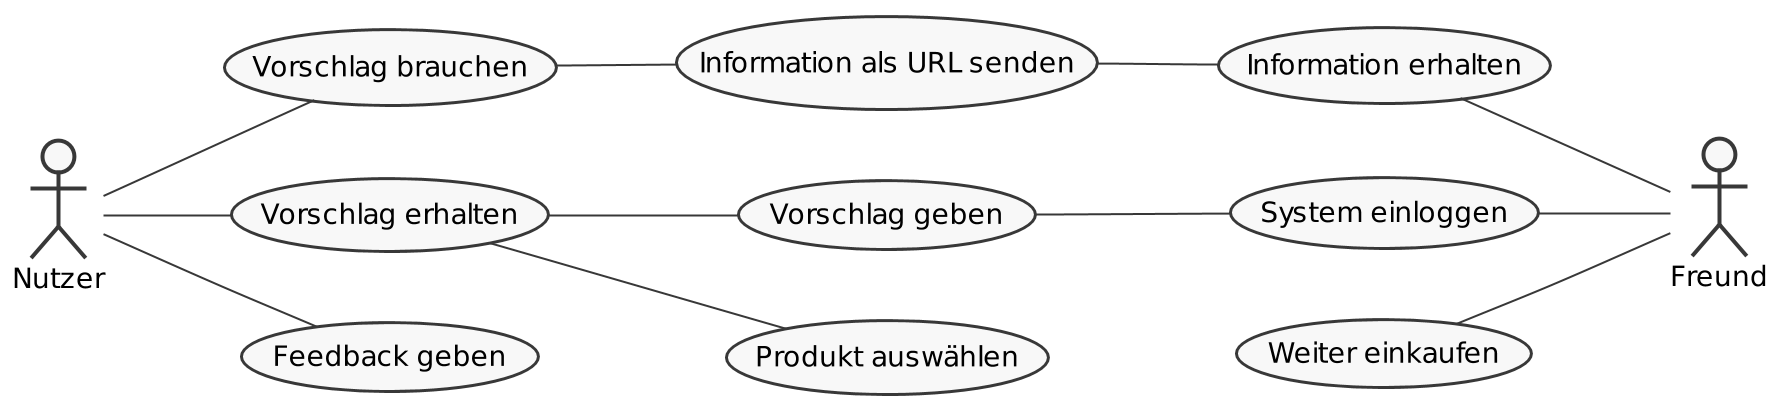
\includegraphics[width=1\textwidth]{uml-diagramme/freunde-einladen.png}
	\caption{Freunde einladen}
	\label{fig:freunde-einladen}
\end{figure}


\newpage

\section{Pay by Others}

\begin{figure}[htbp]
	\centering
	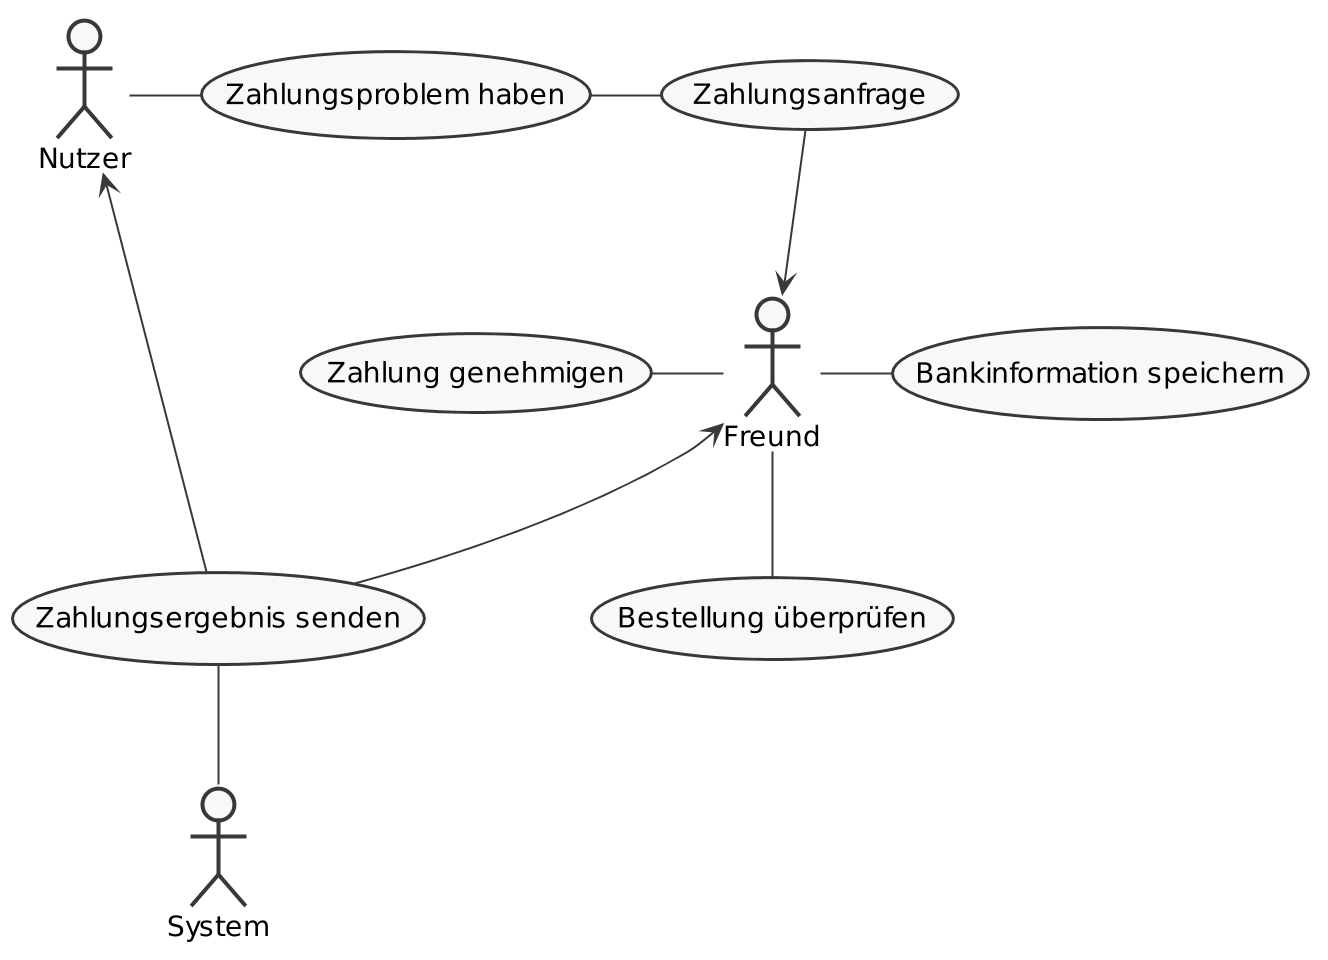
\includegraphics[width=0.8\textwidth]{uml-diagramme/pay-by-others.png}
	\caption{Pay by Others}
	\label{fig:pay-by-others}
\end{figure}


\section{Realtime Kommunikation}

\begin{figure}[htbp]
	\centering
	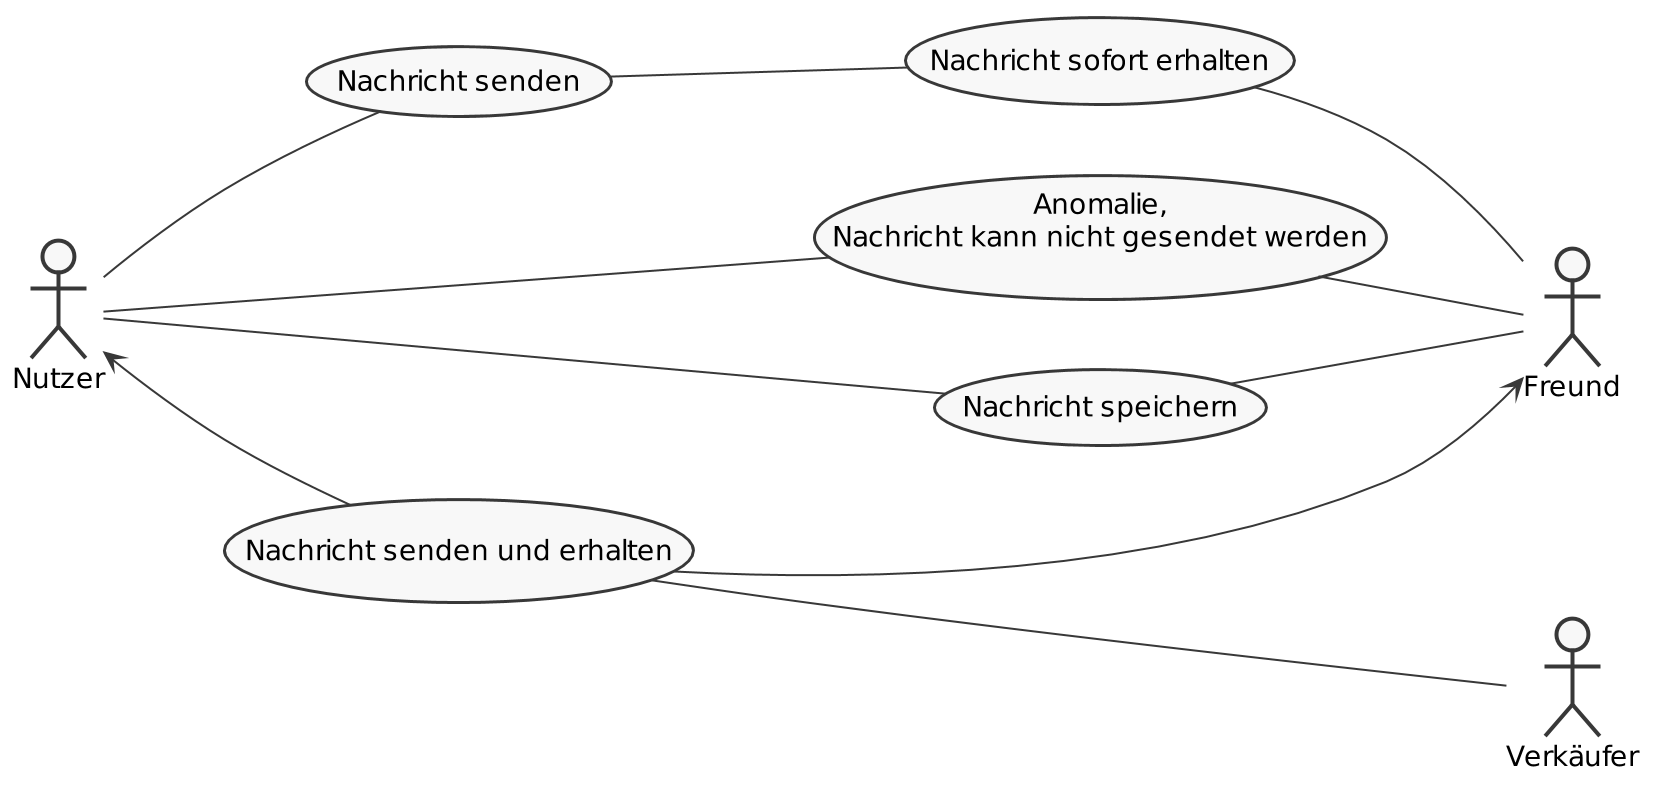
\includegraphics[width=0.8\textwidth]{uml-diagramme/real-time-communication.png}
	\caption{Realtime Kommunikation}
	\label{fig:real-time-communication}
\end{figure}
